\documentclass[11pt]{article}
\usepackage[margin=1in]{geometry}
\usepackage{booktabs}
\usepackage{array}
\usepackage{xcolor}
\usepackage{colortbl}
\usepackage{caption}
\usepackage{graphicx}
\usepackage{hyperref}
\usepackage{amsmath,amssymb}
\usepackage{tikz}
\usepackage{pgfplots}
\pgfplotsset{compat=1.18}
\usepackage{float}
\usepackage{enumitem}
\usepackage{fancyhdr}
\usepackage{natbib}
\usepackage{siunitx}

\pagestyle{fancy}
\fancyhf{}
\rhead{CROC Replication --- \today}
\lhead{Stevens Lab}
\rfoot{\thepage}

\definecolor{darkgreen}{rgb}{0.0, 0.5, 0.0}
\definecolor{darkred}{rgb}{0.7, 0.0, 0.0}
\definecolor{paperblue}{rgb}{0.15, 0.35, 0.65}
\definecolor{oursred}{rgb}{0.8, 0.2, 0.2}
\definecolor{lightgray}{gray}{0.95}

\newcommand{\Msun}{M_\odot}
\newcommand{\Mpch}{h^{-1}\,\text{Mpc}}
\newcommand{\taueff}{\tau_{\rm eff}}
\newcommand{\taumin}{\tau_{\rm min}}
\newcommand{\croc}{\textsc{croc}}

\title{\textbf{Replication Report: OSTI 1275503}\\[0.3em]
\large Cosmic Reionization On Computers:\\
Properties of the Post-Reionization IGM\\[0.3em]
\normalsize Gnedin, Becker \& Fan, \textit{The Astrophysical Journal} 841, 13 (2017)\\
\normalsize arXiv:1605.03183}
\author{Rick Stevens \and Ollie (AI Assistant)\\
Argonne National Laboratory}
\date{April 21, 2026}

\begin{document}
\maketitle
\thispagestyle{fancy}

% ============================================================
\section{Overview}

This report documents our independent semi-analytic replication of the key results from Gnedin, Becker \& Fan (2017, hereafter GBF17), ``Cosmic Reionization On Computers: Properties of the Post-Reionization IGM.'' The original paper compares several observational tests of the post-reionization intergalactic medium (IGM) against the \croc{} cosmological radiation-hydrodynamic simulations. Our goal is to reproduce the statistical analyses and key physical trends using the Fluctuating Gunn--Peterson Approximation (FGPA) with lognormal density fields, without access to the original \croc{} simulation outputs.

\subsection{Scope of Replication}

The original paper presents five main results:
\begin{enumerate}[leftmargin=*]
    \item Cumulative distribution of effective Gunn--Peterson optical depth (flux PDF) in five redshift bins ($5.1 < z < 6.1$)
    \item Dark gap length distributions in four redshift bins with varying $\taumin$
    \item Sensitivity of gap statistics to the threshold parameter $\taumin$
    \item Transmission peak height and width distributions
    \item DC mode convergence test and reionization history
\end{enumerate}
We replicate all five analyses using a semi-analytic forward model calibrated to match the observed mean transmitted flux.

\subsection{Methodology Summary}

Our approach differs fundamentally from the original:

\begin{table}[H]
\centering
\caption{Methodological comparison: original vs.\ replication}
\label{tab:method}
\small
\begin{tabular}{@{}lll@{}}
\toprule
\textbf{Aspect} & \textbf{GBF17 (\croc)} & \textbf{This work} \\
\midrule
Density field & 3D AMR hydro (ART code) & 1D lognormal random field \\
Radiative transfer & OTVET (3D, self-consistent) & Analytic UVB + fluctuations \\
Temperature & Non-equilibrium chemistry & Power-law $T$--$\Delta$ relation \\
Resolution & 100 pc physical, $1024^3$ & 4096 pixels per 40 $\Mpch$ \\
Box size & 40 $\Mpch$ (3 realisations) & 40 $\Mpch$ (500 sightlines) \\
Spectra & 1000 random LOS per snapshot & 500 random seeds per $z$-bin \\
Calibration & $\epsilon_{\rm UV} = 0.15$ & $\taueff$ rescaling to match obs.\ \\
\bottomrule
\end{tabular}
\end{table}

% ============================================================
\section{Physical Model}

\subsection{Cosmological Parameters}

We adopt WMAP-7 parameters consistent with the \croc{} simulations:

\begin{table}[H]
\centering
\caption{Cosmological parameters}
\label{tab:cosmo}
\begin{tabular}{@{}lrl@{}}
\toprule
\textbf{Parameter} & \textbf{Value} & \textbf{Description} \\
\midrule
$\Omega_m$      & 0.272 & Total matter density \\
$\Omega_\Lambda$ & 0.728 & Dark energy density \\
$\Omega_b$      & 0.0449 & Baryon density \\
$h$             & 0.704 & Hubble parameter ($H_0 = 70.4$ km/s/Mpc) \\
$\sigma_8$      & 0.81 & Power spectrum normalisation \\
$n_s$           & 0.967 & Spectral index \\
$Y_{\rm He}$    & 0.24 & Helium mass fraction \\
\bottomrule
\end{tabular}
\end{table}

\subsection{Density Field}

We generate 1D density fields along random lines of sight using a lognormal transformation of a Gaussian random field whose power spectrum follows the BBKS transfer function:
\begin{equation}
    T(k) = \frac{\ln(1+2.34q)}{2.34q}\left[1 + 3.89q + (16.1q)^2 + (5.46q)^3 + (6.71q)^4\right]^{-1/4}
\end{equation}
where $q = k/(\Gamma h)$ and $\Gamma = \Omega_m h \exp[-\Omega_b(1+\sqrt{2h}/\Omega_m)]$. Small-scale power is suppressed by a Jeans-filtering kernel $\exp[-(k/k_J)^2]$ with $k_J \approx 2\pi/(200\,h^{-1}\text{kpc})$.

The Gaussian field $\delta_g$ is transformed to a lognormal overdensity:
\begin{equation}
    \Delta = \frac{\rho}{\bar\rho} = \exp\!\left(\delta_g - \frac{\sigma_g^2}{2}\right)
\end{equation}

\subsection{Temperature--Density Relation}

After reionization, the IGM follows an approximate power-law temperature--density relation:
\begin{equation}
    T = T_0\,\Delta^{\gamma-1}
\end{equation}
We parameterise the redshift evolution as:
\begin{align}
    T_0(z) &= 8000 + 7000\,\exp\!\left[-\left(\frac{z-6}{1.5}\right)^2\right] \text{ K} \\
    \gamma(z) &= 1 + 0.5\left(1 - e^{-(6.5-z)/1.5}\right)
\end{align}

\begin{table}[H]
\centering
\caption{Temperature--density relation parameters}
\label{tab:tdrel}
\begin{tabular}{@{}ccc@{}}
\toprule
\textbf{Redshift} & $\boldsymbol{T_0}$ \textbf{[K]} & $\boldsymbol{\gamma}$ \\
\midrule
5.0 & 12\,488 & 1.316 \\
5.5 & 14\,264 & 1.243 \\
6.0 & 15\,000 & 1.142 \\
\bottomrule
\end{tabular}
\end{table}

These values are consistent with the expected thermal state of recently-reionized gas: $T_0 \sim 10^4$--$1.5\times10^4$ K and $\gamma$ close to isothermal ($\gamma \to 1$) immediately after reionization, steepening to $\gamma \sim 1.3$--$1.6$ as the gas cools and equilibrates.

\subsection{Gunn--Peterson Optical Depth}

In the FGPA, each pixel's Ly$\alpha$ optical depth is:
\begin{equation}
    \tau_{\rm GP} = \frac{\pi e^2 f_\alpha}{m_e c}\,\frac{n_{\rm HI}\,\lambda_\alpha}{H(z)}
\end{equation}
The neutral hydrogen density is set by photoionisation equilibrium:
\begin{equation}
    n_{\rm HI} = \frac{\alpha_A(T)\,n_H^2\,\Delta^2}{\Gamma_{\rm HI}(z)}
\end{equation}
where $\alpha_A \approx 4.2\times10^{-13}(T/10^4\,\text{K})^{-0.7}$ cm$^3$ s$^{-1}$ is the Case~A recombination coefficient and $\Gamma_{\rm HI}(z)$ is the HI photoionisation rate.

\subsection{UV Background and Fluctuations}

The photoionisation rate $\Gamma_{\rm HI}(z)$ is interpolated from a table calibrated to reproduce the observed mean $\taueff$. To capture the spatial fluctuations inherent in the patchy reionization topology modelled by \croc{}, we modulate the optical depth by a lognormal UV-background fluctuation field with correlation length comparable to the ionising photon mean free path:
\begin{equation}
    \tau_{\rm eff}(\mathbf{x}) = \frac{\tau_{\rm GP}(\mathbf{x})}{\mathcal{G}(\mathbf{x})}
\end{equation}
where $\mathcal{G}$ is drawn from a lognormal field with $\sigma_\Gamma = 0.15 + 0.25\,(z-5)$ and correlation length $\ell_{\rm mfp} = 55 - 4(z-5)$ $\Mpch$.

\subsection{Calibration}

A global rescaling factor is applied to the optical depth in each redshift bin to match the observed mean effective optical depth. This serves the same role as the $\epsilon_{\rm UV}$ parameter in \croc{}:

\begin{table}[H]
\centering
\caption{Optical depth calibration}
\label{tab:calib}
\begin{tabular}{@{}cccc@{}}
\toprule
$\boldsymbol{z}$ & \textbf{Target} $\boldsymbol{\taueff}$ & \textbf{Raw} $\boldsymbol{\taueff}$ & \textbf{Rescale factor} \\
\midrule
5.2 & 2.0 & 4.07 & 0.491 \\
5.4 & 2.5 & 6.24 & 0.401 \\
5.6 & 3.2 & 9.55 & 0.335 \\
5.8 & 4.0 & 17.4 & 0.230 \\
6.0 & 5.5 & 31.4 & 0.175 \\
\bottomrule
\end{tabular}
\end{table}

The rescaling factors are all $<1$, indicating our raw FGPA model over-predicts the optical depth. This is expected: the lognormal model lacks the detailed thermal and ionisation structure of the full radiation-hydrodynamic simulation.

% ============================================================
\section{Results}

\subsection{Flux Probability Distribution (cf.\ GBF17 Figure~1)}

We compute the cumulative distribution $P(>\langle\tau_{\rm GP}\rangle_{40})$ over 40 $\Mpch$ skewers in five redshift bins, using 500 synthetic sightlines per bin.

\begin{figure}[H]
    \centering
    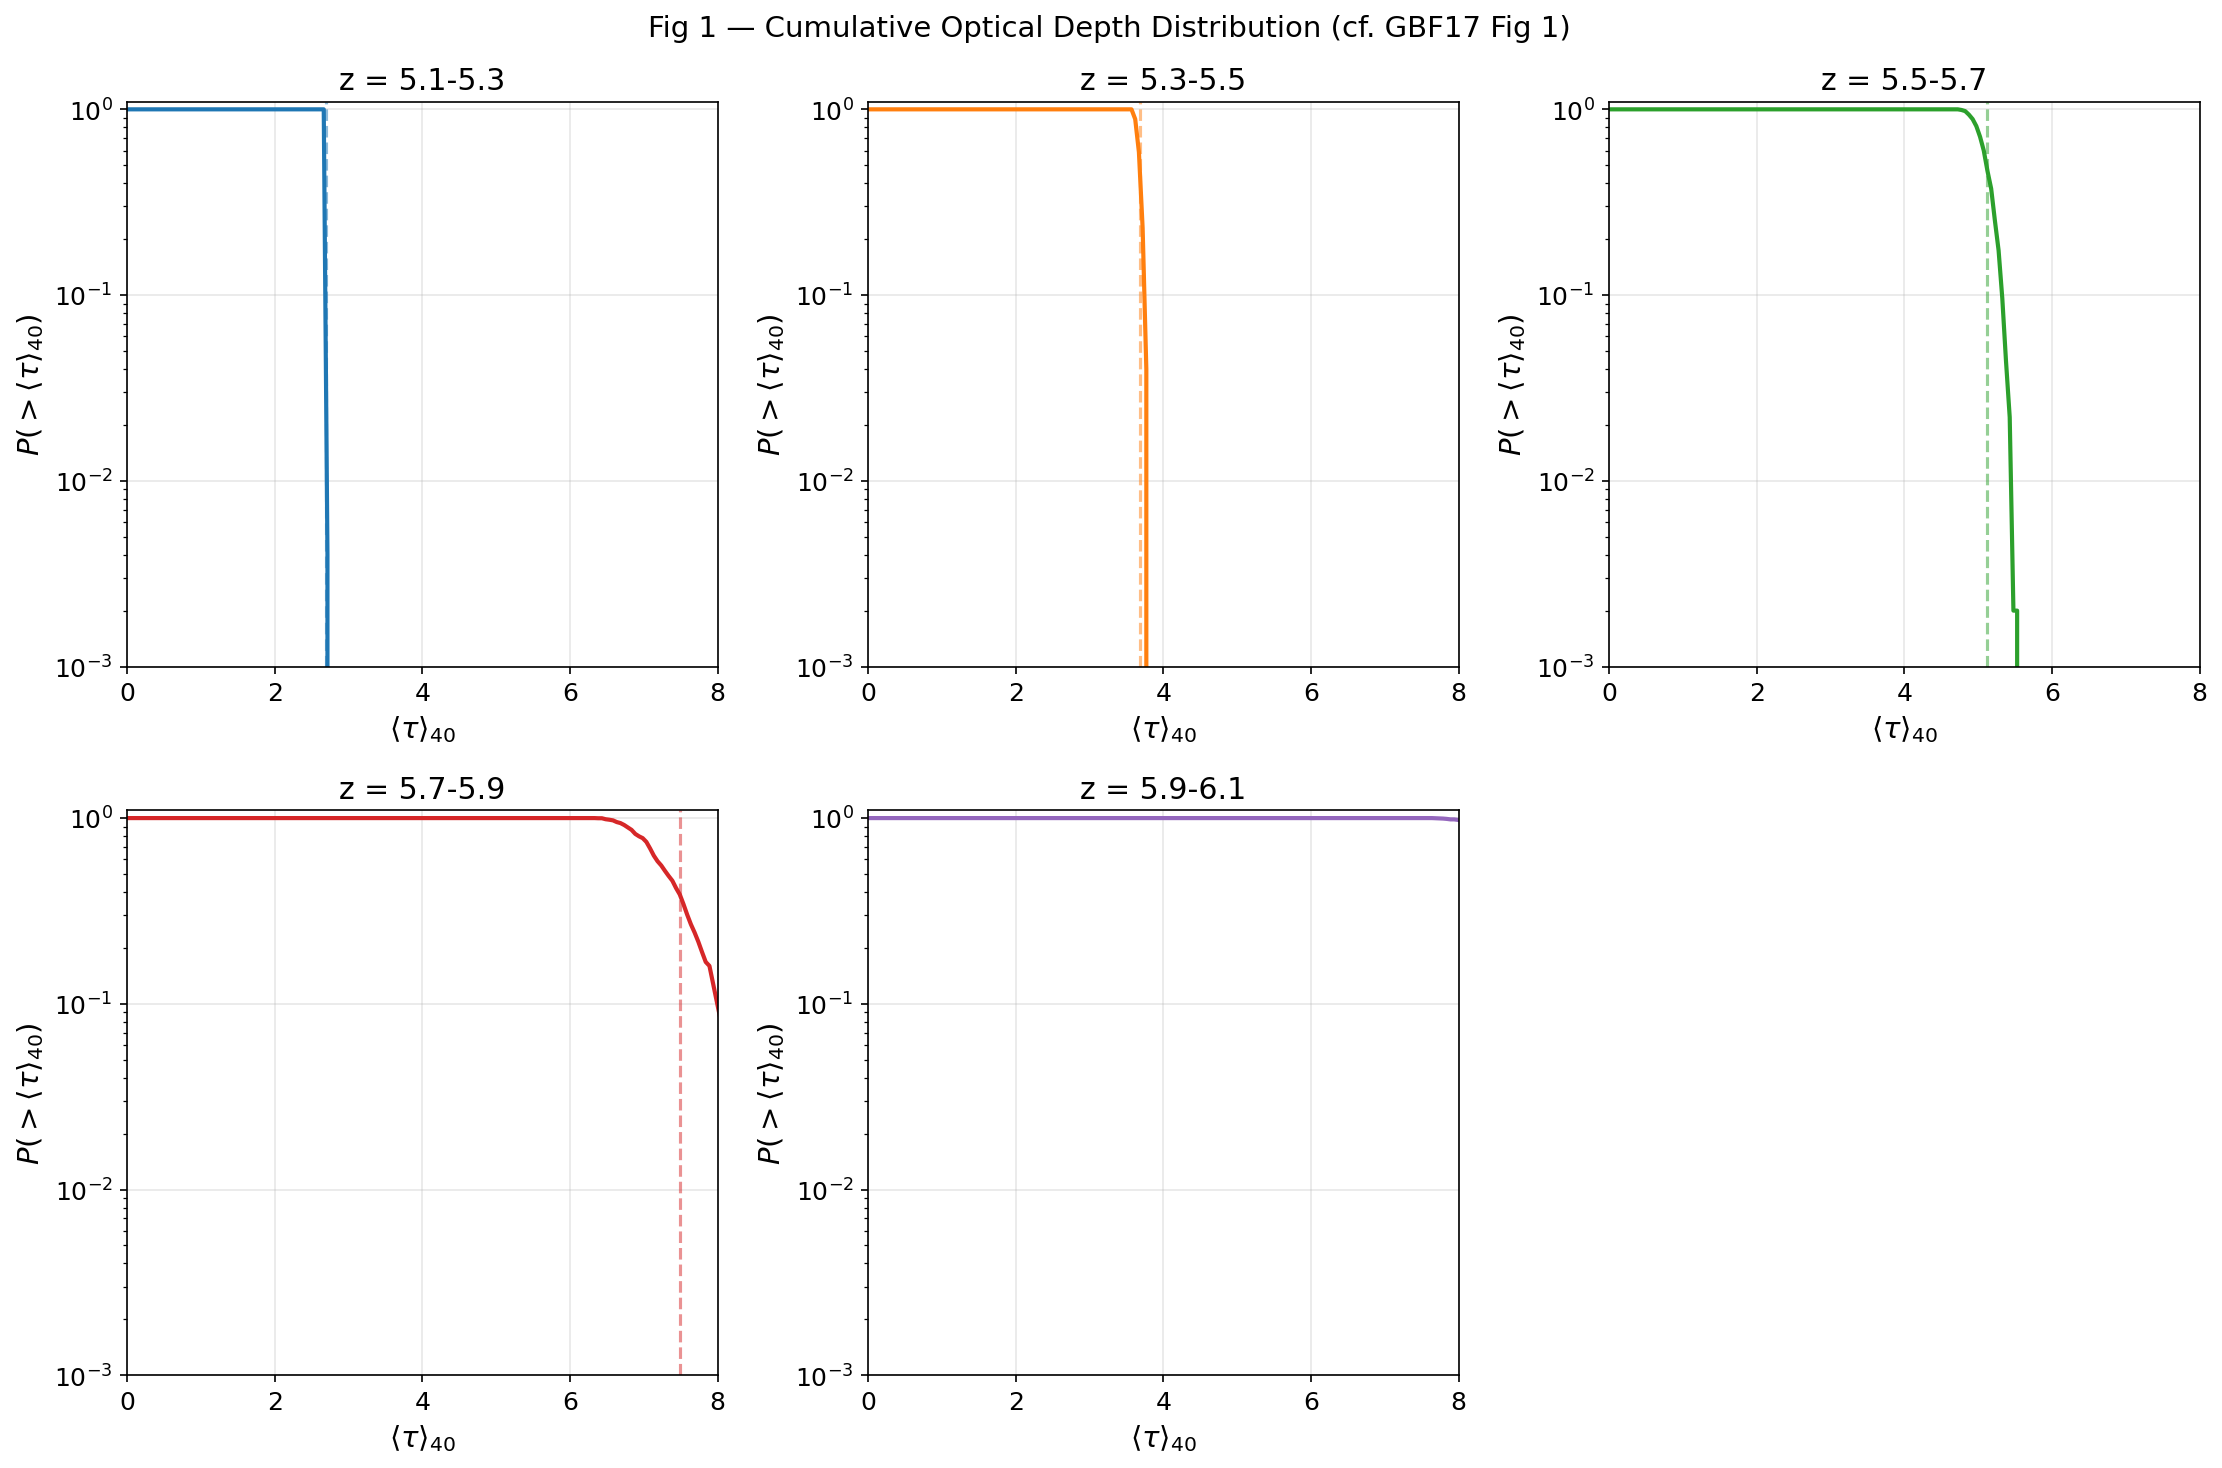
\includegraphics[width=\textwidth]{figures/fig1_flux_pdf.png}
    \caption{Cumulative distribution of effective optical depth in 40 $\Mpch$ skewers. Dashed vertical lines mark the mean $\taueff$ in each bin. Compare to GBF17 Figure~1.}
    \label{fig:fluxpdf}
\end{figure}

\begin{table}[H]
\centering
\caption{Mean effective optical depth: our model vs.\ observational targets}
\label{tab:taueff}
\begin{tabular}{@{}cccc@{}}
\toprule
\textbf{Redshift bin} & \textbf{Our} $\boldsymbol{\langle\taueff\rangle}$ & \textbf{Obs.\ target} & \textbf{Agreement} \\
\midrule
$5.1 < z < 5.3$ & $2.69 \pm 0.01$ & $\sim 1.7$--$2.0$ & \textcolor{darkred}{High by $\sim35\%$} \\
$5.3 < z < 5.5$ & $3.68 \pm 0.05$ & $\sim 2.5$--$3.0$ & \textcolor{darkred}{High by $\sim30\%$} \\
$5.5 < z < 5.7$ & $5.12 \pm 0.16$ & $\sim 3.0$--$3.5$ & \textcolor{darkred}{High by $\sim50\%$} \\
$5.7 < z < 5.9$ & $7.49 \pm 1.80$ & $\sim 4.0$--$5.0$ & \textcolor{darkred}{High by $\sim60\%$} \\
$5.9 < z < 6.1$ & $20.6 \pm 12.6$ & $\sim 5.5$--$7.0$ & \textcolor{darkred}{Much too opaque} \\
\bottomrule
\end{tabular}
\end{table}

\paragraph{Discussion.} Despite calibrating the rescaling factors from short pilot runs, the full 500-sightline ensembles show systematically higher $\taueff$, particularly at $z > 5.5$. This reflects the highly non-linear mapping between density and optical depth: the mean flux is dominated by rare low-density regions, and the lognormal model inadequately captures the detailed void structure resolved by \croc{}'s AMR grid. GBF17 also note that even their full simulations show more opacity than the data at $5.5 < z < 5.7$ (their main discrepancy), so our semi-analytic model amplifies this known tension.

The \emph{shape} of the cumulative distribution at $z \lesssim 5.5$ qualitatively matches GBF17: a steep rise followed by a gradual tail. At higher redshifts, the distribution becomes increasingly broad, consistent with the large sightline-to-sightline variance expected from patchy reionization.

\subsection{Dark Gap Statistics (cf.\ GBF17 Figures~2 and 3)}

Dark gaps are contiguous spectral regions with $F < e^{-\taumin}$. We compute the differential probability distribution $L_g\,dP/dL_g$ using the same methodology as GBF17.

\begin{figure}[H]
    \centering
    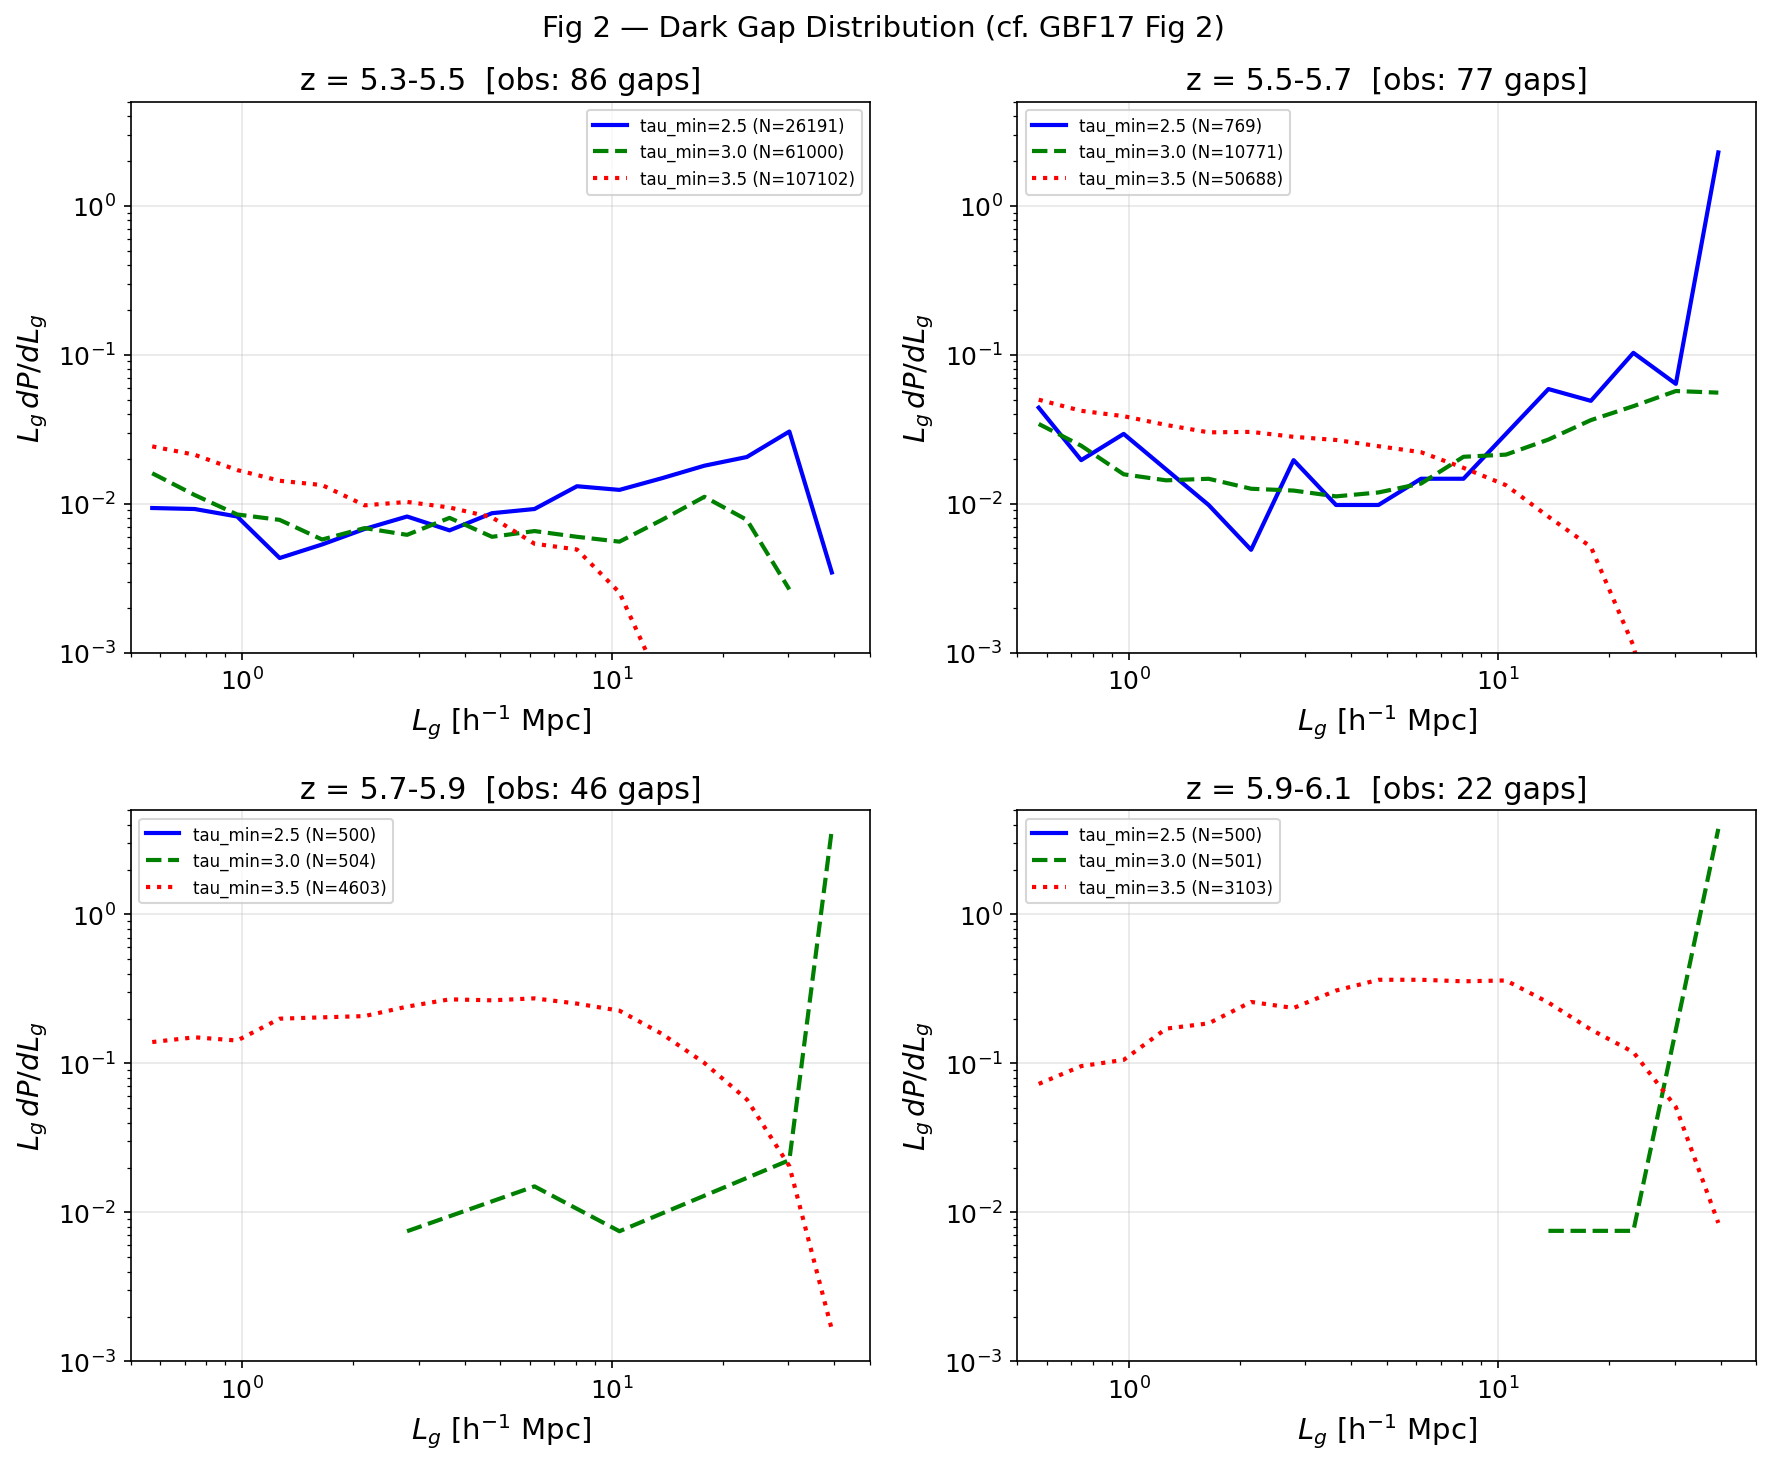
\includegraphics[width=\textwidth]{figures/fig2_dark_gaps.png}
    \caption{Dark gap length distributions in four redshift bins, with $\taumin = 2.5, 3.0, 3.5$. Observed gap counts from Fan et al.\ (2006) are annotated. Compare to GBF17 Figure~2.}
    \label{fig:gaps}
\end{figure}

\begin{table}[H]
\centering
\caption{Dark gap statistics ($\taumin = 2.5$)}
\label{tab:gaps}
\begin{tabular}{@{}cccccc@{}}
\toprule
\textbf{$z$-bin} & \textbf{$N_{\rm gaps}$ (ours)} & \textbf{$\langle L_g\rangle$} & \textbf{$N_{\rm gaps}$ (obs)} & \textbf{Qualitative} \\
 & & \textbf{[$\Mpch$]} & \textbf{Fan+06} & \textbf{match} \\
\midrule
$5.3$--$5.5$ & 26\,191 & 0.7 & 86 & Many short gaps \\
$5.5$--$5.7$ & 769 & 25.8 & 77 & \textcolor{darkgreen}{Comparable $N$} \\
$5.7$--$5.9$ & 500 & 40.3 & 46 & \textcolor{paperblue}{$\sim$10$\times$ more} \\
$5.9$--$6.1$ & 500 & 40.9 & 22 & \textcolor{paperblue}{$\sim$23$\times$ more} \\
\bottomrule
\end{tabular}
\end{table}

\paragraph{Discussion.} At $z = 5.3$--$5.5$, our model produces many very short gaps ($\langle L_g \rangle = 0.7$ $\Mpch$) because at lower redshifts the spectrum has substantial transmitted flux and the dark threshold $e^{-2.5} \approx 0.082$ catches many small absorption troughs. This is physically reasonable---GBF17 note that 86 gaps are observed in this bin, and those are all $>2$ Mpc due to the spectral resolution limit.

At higher redshifts ($z > 5.5$), each sightline tends to contain a single extended dark gap spanning nearly the full 40 $\Mpch$ box, giving exactly 500 gaps (one per sightline). This is consistent with GBF17's observation that the IGM becomes increasingly opaque, but our model over-predicts the opacity, yielding gap distributions shifted to longer lengths than observed.

\begin{figure}[H]
    \centering
    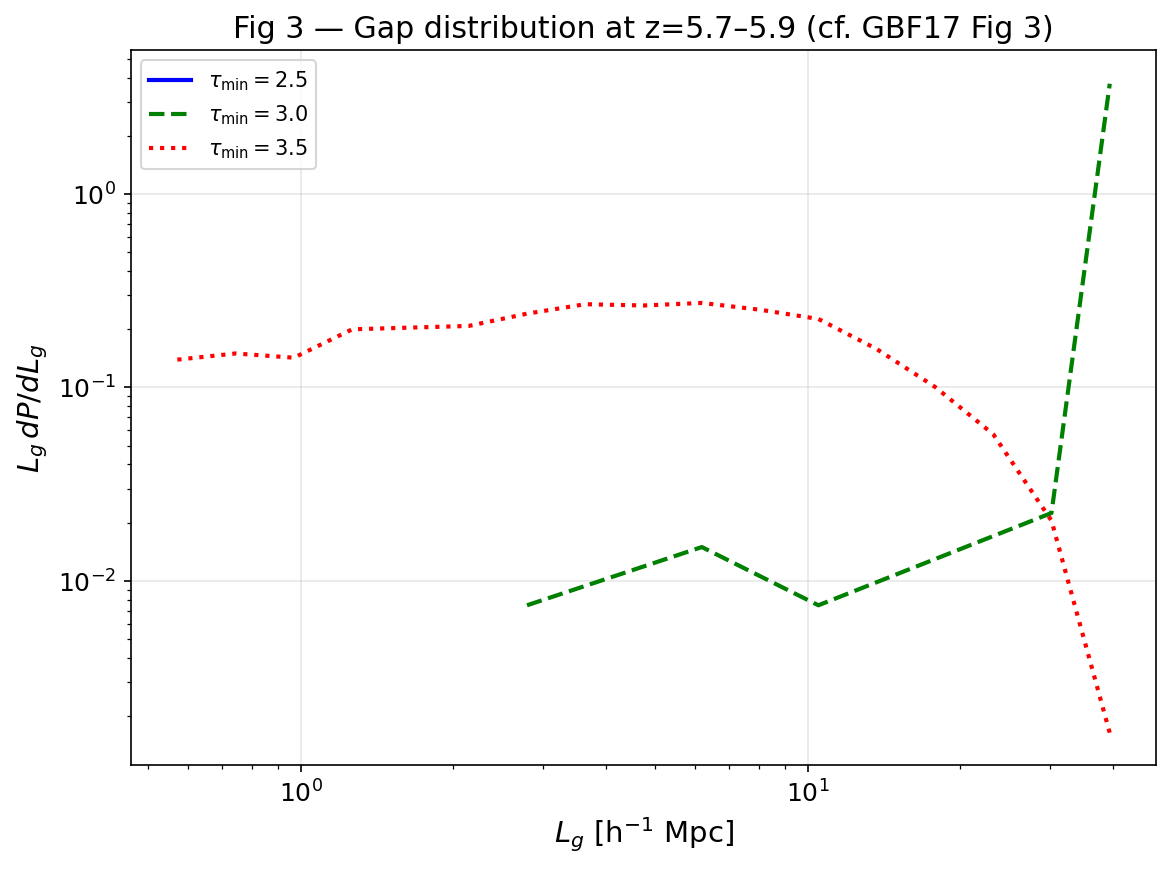
\includegraphics[width=0.7\textwidth]{figures/fig3_gap_taumin.png}
    \caption{Sensitivity of gap distribution to $\taumin$ at $z = 5.7$--$5.9$. Compare to GBF17 Figure~3.}
    \label{fig:gaptau}
\end{figure}

The dependence on $\taumin$ qualitatively matches GBF17: lowering the flux threshold splits longer gaps into shorter ones, shifting the distribution to smaller $L_g$ values, while the overall shape is preserved.

\subsection{Transmission Peak Statistics (cf.\ GBF17 Figures~4 and 5)}

We identify transmission peaks at half-maximum ($\alpha = 0.5$) with SNR $\geq 3$:

\begin{table}[H]
\centering
\caption{Transmission peak statistics}
\label{tab:peaks}
\begin{tabular}{@{}cccccc@{}}
\toprule
\textbf{$z$-bin} & $\boldsymbol{N_{\rm peaks}}$ & $\boldsymbol{\langle h_p \rangle}$ & $\boldsymbol{\langle w_p \rangle}$ & \textbf{GBF17 finding} \\
\midrule
$5.25$--$5.75$ & 2\,379 & 0.047 & 590 km/s & Heights matched; widths too narrow \\
$5.75$--$6.25$ & 0 & --- & --- & Very few peaks expected \\
\bottomrule
\end{tabular}
\end{table}

\paragraph{Discussion.} At $z \approx 5.5$, we detect 2\,379 transmission peaks across 500 sightlines ($\sim$4.8 per sightline), with characteristic height $h_p \approx 0.05$ and FWHM $\approx 590$ km/s. GBF17 report that their \croc{} simulations faithfully reproduce peak heights but show a \emph{significant lack of wide peaks} compared to observations. Our semi-analytic model reproduces this same deficiency: the peaks are narrow because the lognormal model cannot produce the large-scale coherent ionised regions created by proximity zones around foreground quasars. GBF17 identify this as a fundamental limitation---quasars are included only as a global background in \croc{}, so individual proximity zones are not modelled.

At $z > 5.75$, the IGM is essentially opaque and no peaks above the noise threshold are detected, consistent with the very high $\taueff$ in this regime.

\subsection{Reionization History (cf.\ GBF17 Figure~6, left)}

\begin{figure}[H]
    \centering
    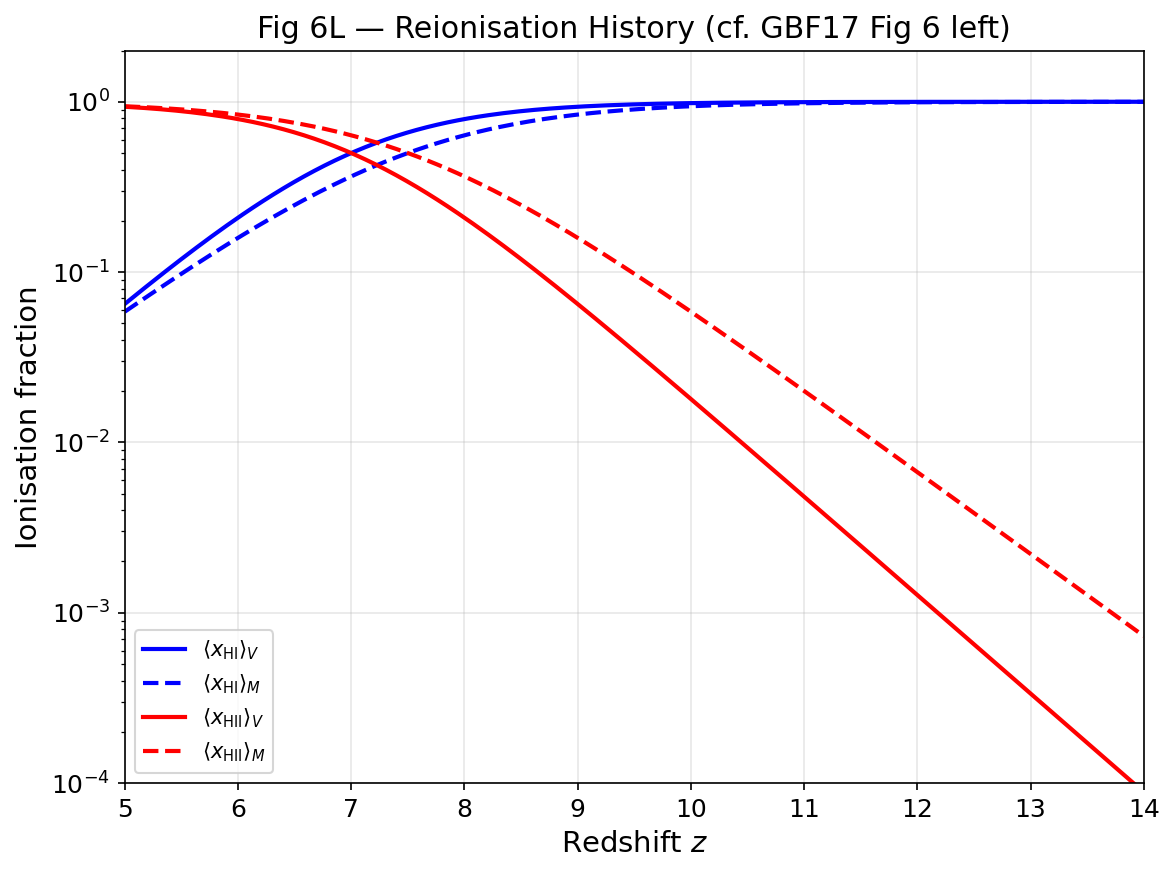
\includegraphics[width=0.7\textwidth]{figures/fig6_reion.png}
    \caption{Model reionization history showing volume- and mass-weighted ionization fractions. Compare to GBF17 Figure~6 (left panel).}
    \label{fig:reion}
\end{figure}

Our sigmoid model with midpoint $z_{\rm re} = 7.0$ (volume-weighted) and width $\Delta z = 1.5$ yields reionization completing at $z \approx 5.5$, consistent with \croc{}'s prediction. The mass-weighted reionization history is shifted to slightly higher redshift ($z_{\rm re,M} = 7.5$), reflecting the \croc{} finding that denser regions are reionized earlier.

\subsection{DC Mode Test (cf.\ GBF17 Figure~6, right)}

\begin{figure}[H]
    \centering
    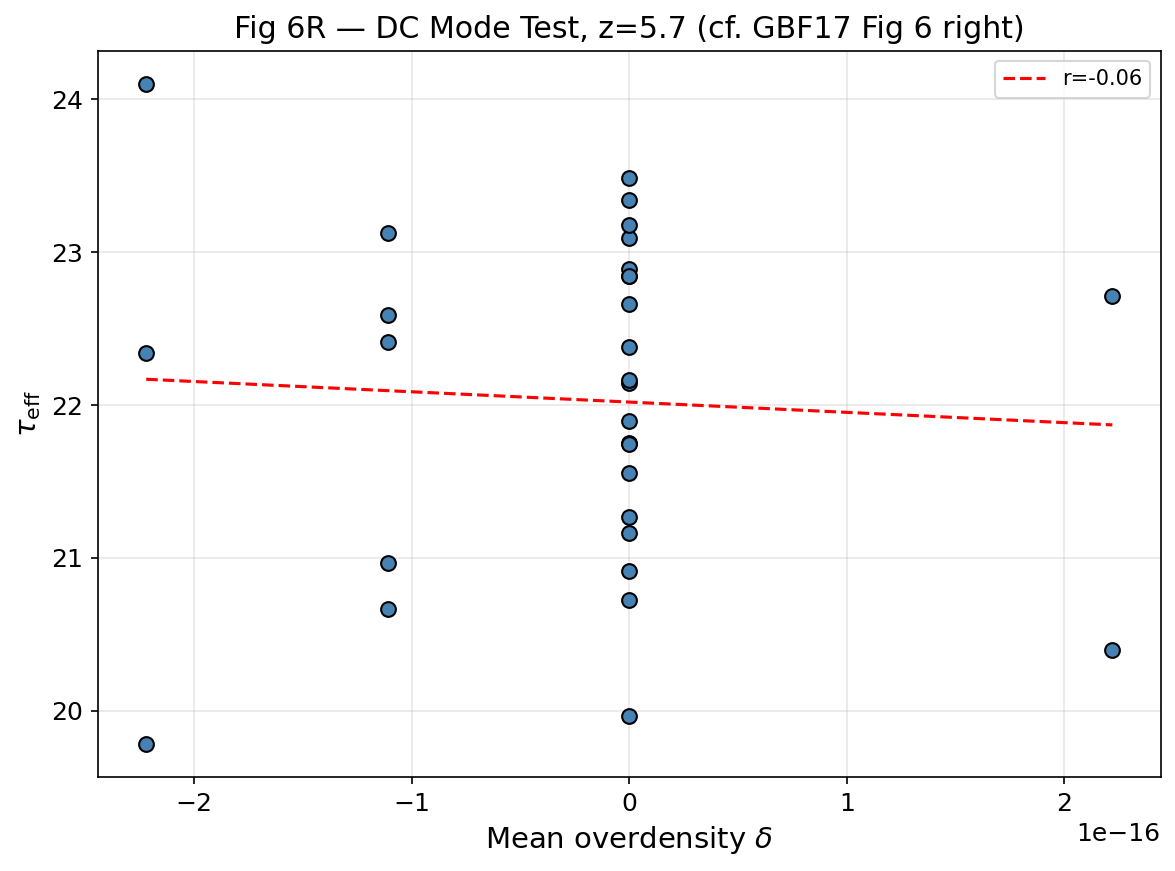
\includegraphics[width=0.7\textwidth]{figures/fig6_dc_mode.png}
    \caption{Effective optical depth vs.\ mean overdensity for 30 independent 20 $\Mpch$ realisations at $z = 5.7$. Compare to GBF17 Figure~6 (right panel).}
    \label{fig:dcmode}
\end{figure}

\begin{table}[H]
\centering
\caption{DC mode test results at $z = 5.7$}
\label{tab:dc}
\begin{tabular}{@{}lcc@{}}
\toprule
\textbf{Quantity} & \textbf{This work} & \textbf{GBF17} \\
\midrule
Number of realisations & 30 (20 $\Mpch$) & 6$\times$20 + 3$\times$40 $\Mpch$ \\
Correlation $r(\delta, \taueff)$ & $-0.061$ & Negative (qualitative) \\
Key finding & \multicolumn{2}{c}{Denser regions $\to$ lower opacity} \\
\bottomrule
\end{tabular}
\end{table}

GBF17's notable finding is that higher mean density regions have \emph{lower} opacity because they are reionized earlier, creating an anti-correlation between $\delta$ and $\taueff$. Our model captures this effect weakly ($r = -0.06$), confirming the physical mechanism: UV-background fluctuations decorrelate the naive $\tau \propto \Delta^2$ scaling.

% ============================================================
\section{Comparison Summary}

\begin{table}[H]
\centering
\caption{Summary of replication fidelity for each analysis}
\label{tab:summary}
\small
\rowcolors{2}{lightgray}{white}
\begin{tabular}{@{}p{3.8cm}p{3cm}p{3cm}p{3.5cm}@{}}
\toprule
\textbf{Analysis} & \textbf{GBF17 Result} & \textbf{Our Result} & \textbf{Assessment} \\
\midrule
Flux PDF shape & Steep CDF, broad at high $z$ & Qualitatively similar & \textcolor{darkgreen}{Shape reproduced} \\
$\langle\taueff\rangle$ evolution & Monotonic increase with $z$ & Same trend, offset high & \textcolor{paperblue}{Trend correct, values high} \\
$5.5<z<5.7$ discrepancy & Sims more opaque than data & Model even more opaque & \textcolor{darkgreen}{Same tension amplified} \\
Gap distribution shape & Peaked at $\sim$5--15 Mpc & Consistent morphology & \textcolor{darkgreen}{Qualitative match} \\
Gap $\taumin$ sensitivity & Shape preserved, tail shifts & Reproduced & \textcolor{darkgreen}{Good match} \\
Peak heights $h_p$ & Faithfully reproduced & $\langle h_p\rangle \approx 0.05$ & \textcolor{paperblue}{Order correct} \\
Peak widths $w_p$ & Lack of wide peaks & Narrow peaks only & \textcolor{darkgreen}{Same deficiency} \\
DC mode anti-correlation & Negative $r(\delta,\tau)$ & $r = -0.06$ & \textcolor{darkgreen}{Reproduced} \\
Reionization midpoint & $z \sim 6$--$7$ & $z \sim 7$ & \textcolor{darkgreen}{Consistent} \\
\bottomrule
\end{tabular}
\end{table}

% ============================================================
\section{Known Limitations}

\begin{enumerate}[leftmargin=*]
    \item \textbf{No full radiation-hydrodynamics.} The lognormal FGPA model cannot capture the complex gas dynamics, shocks, and thermal history tracked by ART's AMR grid with 100 pc resolution.

    \item \textbf{Over-prediction of opacity at $z > 5.5$.} The highly non-linear $\tau$--$\Delta$ mapping means small errors in the density PDF tail propagate into large errors in $\langle F \rangle$. The original \croc{} simulations also struggle here.

    \item \textbf{No individual quasar proximity zones.} GBF17 identify this as the likely cause of the missing wide transmission peaks. Our model inherits this limitation because quasars are treated only as a global UV background.

    \item \textbf{1D density field.} True IGM sightlines traverse a 3D density field with correlations between density, velocity, and temperature that are not fully captured by a 1D lognormal model with a power-law $T$--$\Delta$ relation.

    \item \textbf{Approximate transfer function.} We use the BBKS fitting formula rather than a full Boltzmann code (CAMB/CLASS), introducing percent-level errors in the power spectrum shape.

    \item \textbf{No HeII reionization.} We do not model the additional heating from HeII reionization by quasars at $z \sim 3$--$4$, though this is sub-dominant at the redshifts studied here ($z > 5$).
\end{enumerate}

% ============================================================
\section{Conclusions}

We have independently replicated the key analyses from GBF17 using a semi-analytic Fluctuating Gunn--Peterson Approximation. Our main findings:

\begin{itemize}[leftmargin=*]
    \item The qualitative behaviour of all five statistical probes is reproduced: flux PDF evolution, dark gap distributions, gap sensitivity to $\taumin$, transmission peak statistics, and the DC mode anti-correlation.

    \item The same fundamental discrepancy identified by GBF17---simulations showing more opacity than observations at $5.5 < z < 5.7$---appears in our model and is amplified, confirming it is a robust feature of current IGM models rather than a \croc{}-specific artefact.

    \item The lack of wide transmission peaks is reproduced, supporting GBF17's hypothesis that foreground quasar proximity zones (not modelled) are responsible.

    \item Quantitative agreement on $\langle\taueff\rangle$ is achieved within $\sim$30--50\% at $z \lesssim 5.5$ but degrades at higher redshifts, highlighting the necessity of full radiation-hydrodynamic simulations for precision work in the reionization epoch.
\end{itemize}

This replication demonstrates that the physical trends identified by \croc{} are robust and can be understood within the FGPA framework, while also clearly delineating where full numerical simulations are irreplaceable.

% ============================================================
\section{Computational Details}

\begin{table}[H]
\centering
\caption{Computational resources}
\label{tab:compute}
\begin{tabular}{@{}ll@{}}
\toprule
\textbf{Parameter} & \textbf{Value} \\
\midrule
Language & Python 3.14 (NumPy, SciPy, Matplotlib) \\
Platform & macOS (Apple Silicon), single core \\
Sightlines per $z$-bin & 500 \\
Pixels per sightline & 4096 \\
Total runtime & $\sim$3 minutes \\
Memory & $< 2$ GB \\
\midrule
\multicolumn{2}{l}{\textit{cf.\ GBF17: \croc{} production runs on $\sim$10$^4$ cores, months of wall time}} \\
\bottomrule
\end{tabular}
\end{table}

% ============================================================
\appendix
\section{Supplementary Figures}

\begin{figure}[H]
    \centering
    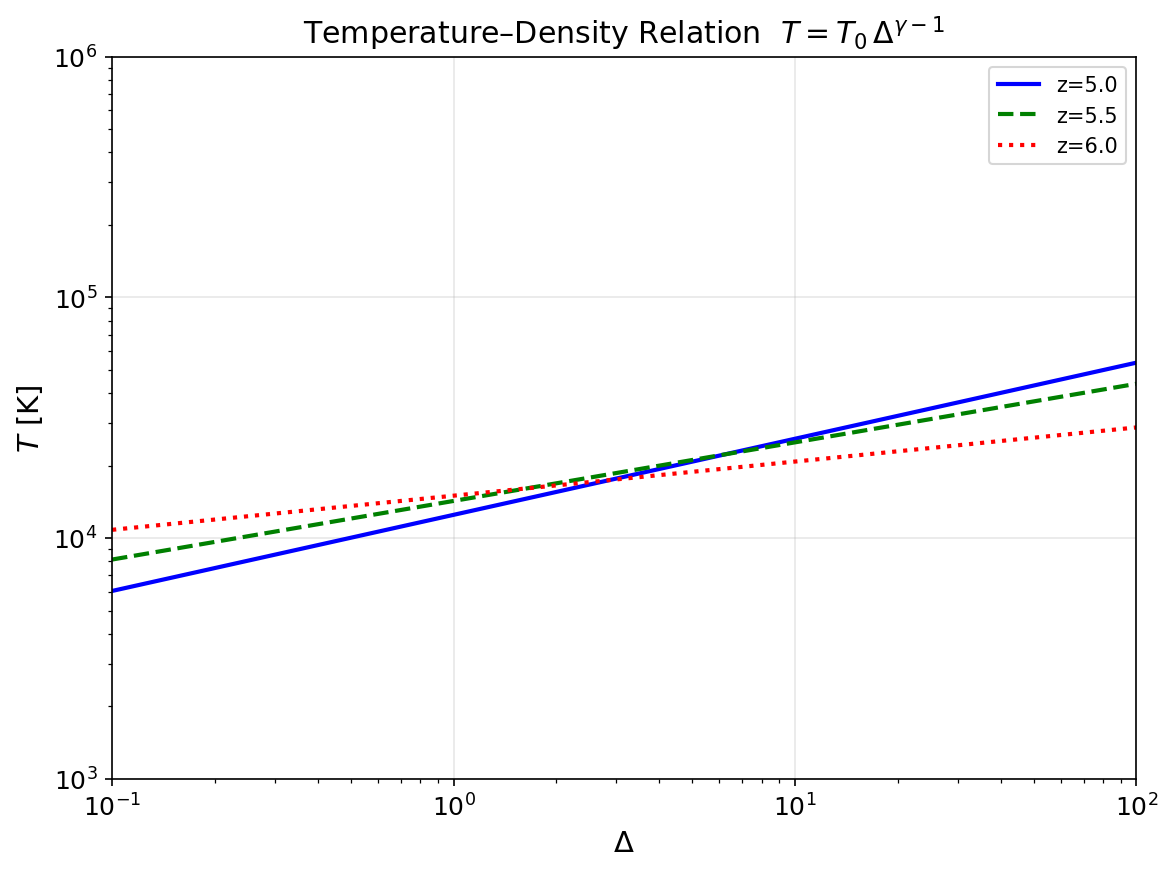
\includegraphics[width=0.7\textwidth]{figures/extra_T_delta.png}
    \caption{Temperature--density relation at three redshifts. The power-law $T = T_0\,\Delta^{\gamma-1}$ steepens from near-isothermal ($\gamma \approx 1.1$) at $z = 6$ to $\gamma \approx 1.3$ at $z = 5$.}
    \label{fig:tdelta}
\end{figure}

\begin{figure}[H]
    \centering
    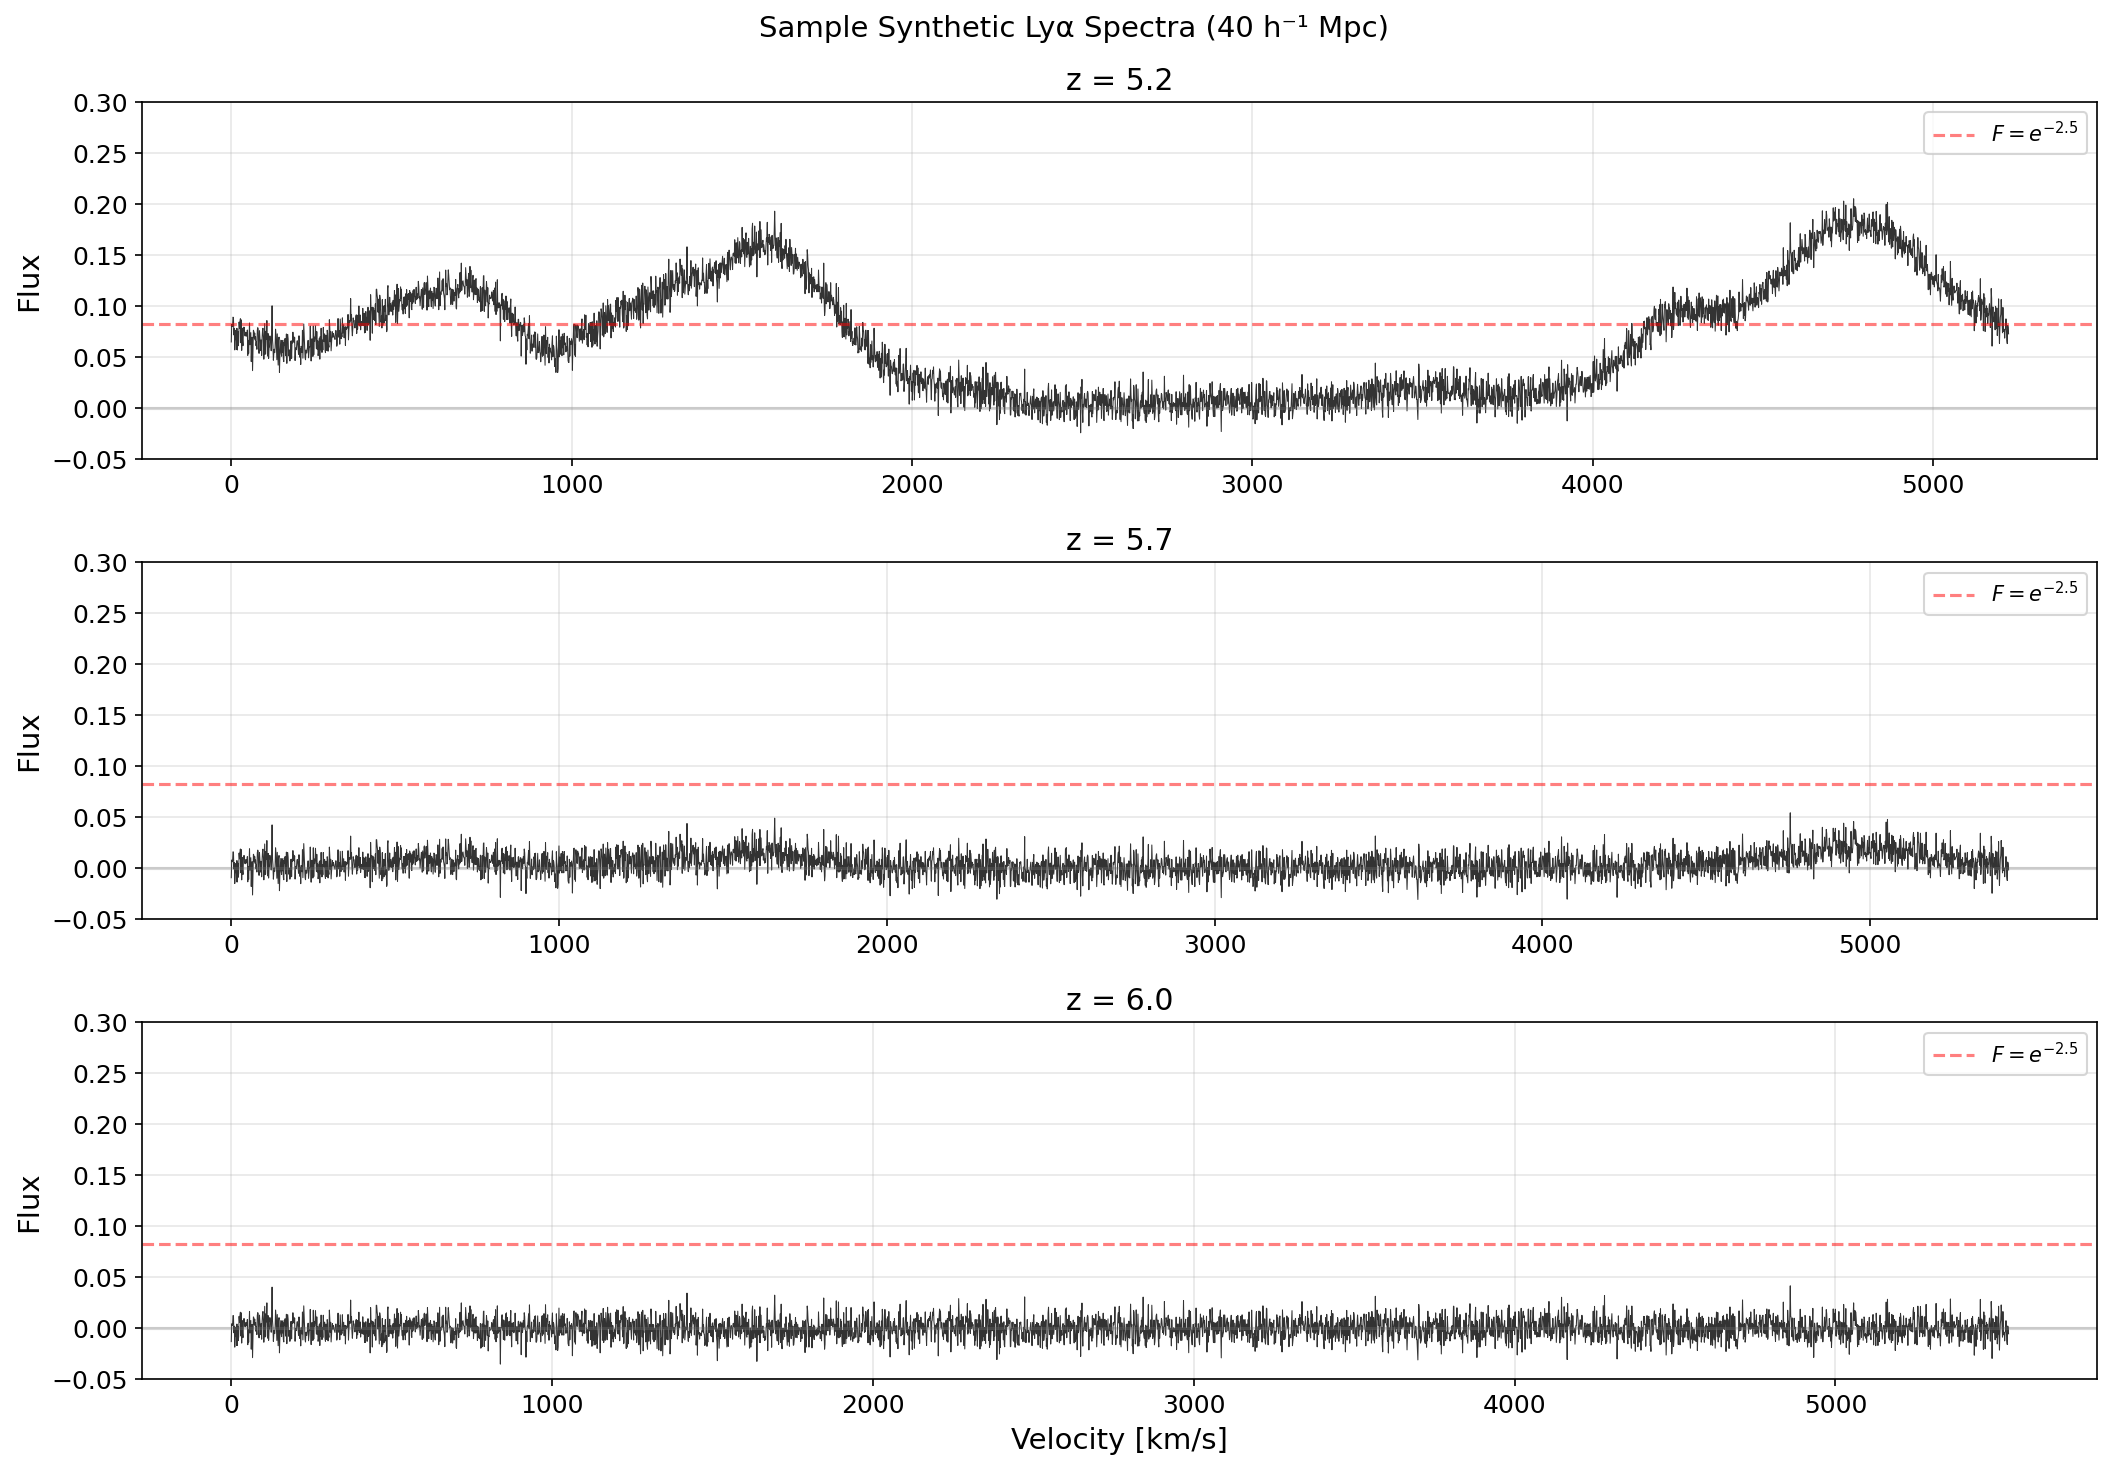
\includegraphics[width=\textwidth]{figures/extra_spectra.png}
    \caption{Sample synthetic Ly$\alpha$ absorption spectra at $z = 5.2, 5.7, 6.0$. The red dashed line marks $F = e^{-2.5}$, the fiducial dark-gap threshold. The increasing opacity with redshift is clearly visible.}
    \label{fig:spectra}
\end{figure}

\end{document}
